\documentclass[11pt]{article}

% ============================================================================
%  Equation (1): the simplified "proof space" structure
%  Module DAG, the classifier equivalence, the parity graph, and the
%  engine-free / engine split of the headline criterion.
% ============================================================================

\usepackage[a4paper,margin=2.2cm]{geometry}
\usepackage{amsmath,amssymb,amsthm}
\usepackage{xcolor}
\usepackage{graphicx}
\usepackage{tikz}
\usetikzlibrary{arrows.meta,positioning,shapes.geometric,fit,backgrounds,calc}
\usepackage{tikz-cd}
\usepackage{enumitem}
\usepackage[hidelinks]{hyperref}
\usepackage{fontspec}
\setmonofont{DejaVu Sans Mono}

\definecolor{mathlibcol}{RGB}{215,232,255}
\definecolor{fieldcol}{RGB}{222,245,222}
\definecolor{numcol}{RGB}{224,240,255}
\definecolor{mapcol}{RGB}{255,244,214}
\definecolor{critcol}{RGB}{235,225,255}
\definecolor{headcol}{RGB}{255,224,224}
\definecolor{spacecol}{RGB}{224,244,240}

\newcommand{\lst}[1]{{\small\texttt{#1}}}
\newcommand{\Fq}{\mathbb{F}_{2^{n}}}
\newcommand{\Zmod}{\mathbb{Z}/2\mathbb{Z}}

\theoremstyle{definition}
\newtheorem*{obs}{Observation}

\title{\bfseries Equation (1): the simplified proof-space structure\\[2pt]
\large Module DAG, the classifier equivalence, and the parity graph}
\author{}
\date{}

\begin{document}
\maketitle
\vspace{-2.2em}

\begin{center}
\small A companion to \lst{docs/Equation1\_Shortcuts\_and\_Redundancies.md}.
All declarations named here build and are \lst{sorry}-free on the standard
axioms \lst{propext}, \lst{Classical.choice}, \lst{Quot.sound}.
\end{center}

\section{The module dependency DAG (new modules highlighted)}

The Kasami permutation-criterion library, with the two new ``proof space''
modules (\lst{Equation1ProofSpace}, \lst{Equation1Classifier}) drawn in teal.
An arrow $A\to B$ means ``$B$ imports $A$''.

\begin{center}
\resizebox{\textwidth}{!}{%
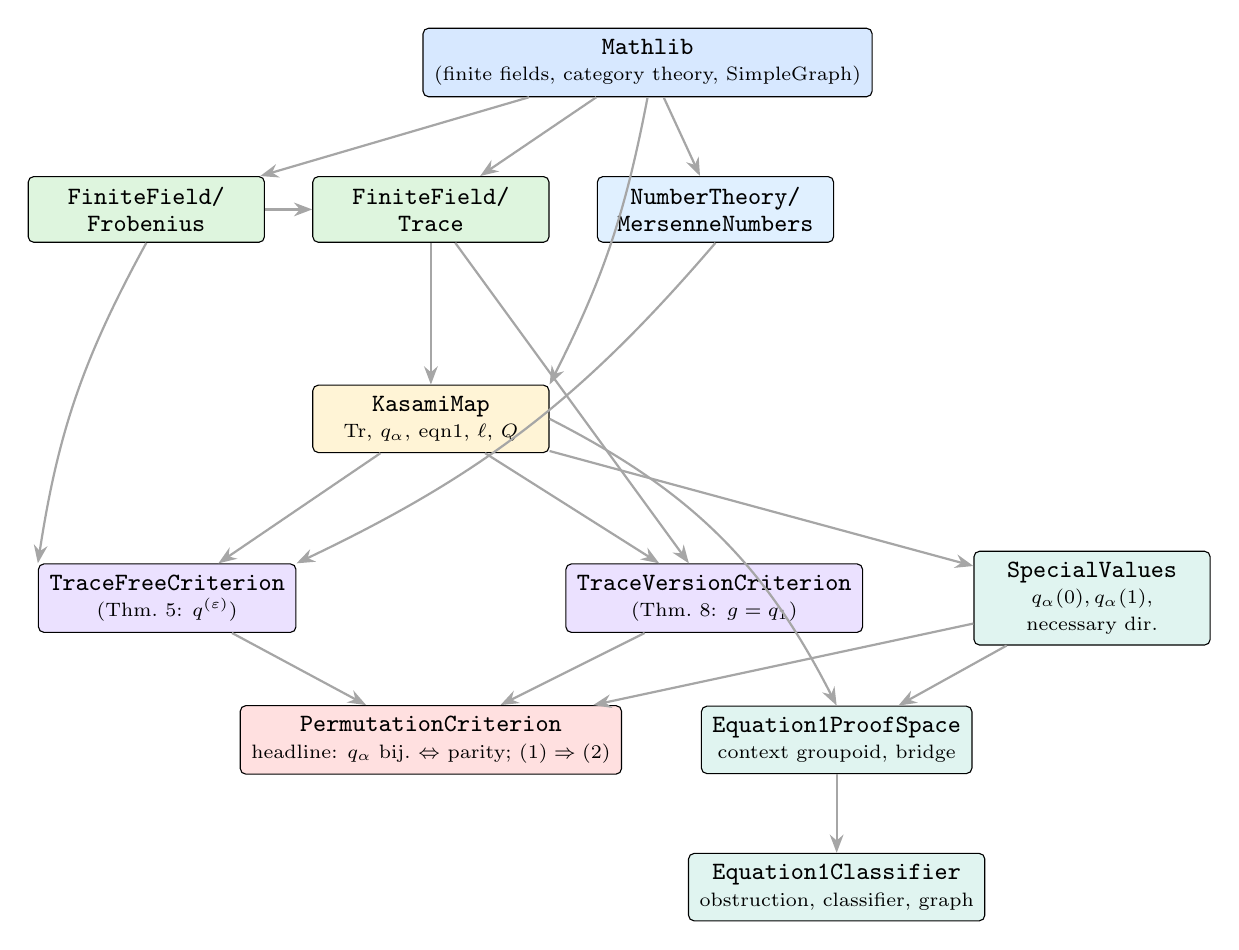
\begin{tikzpicture}[
    >=Stealth, node distance=6mm,
    box/.style={draw, rounded corners=2pt, align=center, inner sep=4pt,
                font=\footnotesize, minimum height=8mm, minimum width=30mm},
    ml/.style={box, fill=mathlibcol},
    ff/.style={box, fill=fieldcol},
    nt/.style={box, fill=numcol},
    mp/.style={box, fill=mapcol},
    cr/.style={box, fill=critcol},
    hd/.style={box, fill=headcol},
    sp/.style={box, fill=spacecol},
    ar/.style={->, thick, gray!70}
  ]
  \node[ml] (mathlib) {\lst{Mathlib}\\ \scriptsize (finite fields, category theory, SimpleGraph)};

  \node[ff, below left=10mm and 20mm of mathlib] (frob) {\lst{FiniteField/}\\\lst{Frobenius}};
  \node[ff, right=6mm of frob] (trace) {\lst{FiniteField/}\\\lst{Trace}};
  \node[nt, right=6mm of trace] (mers) {\lst{NumberTheory/}\\\lst{MersenneNumbers}};

  \node[mp, below=18mm of trace] (kmap) {\lst{KasamiMap}\\ \scriptsize $\mathrm{Tr},\,q_\alpha,\,\mathrm{eqn1},\,\ell,\,Q$};

  \node[cr, below left=14mm and 2mm of kmap] (tfc) {\lst{TraceFreeCriterion}\\ \scriptsize (Thm.\ 5: $q^{(\varepsilon)}$)};
  \node[cr, below right=14mm and 2mm of kmap] (tvc) {\lst{TraceVersionCriterion}\\ \scriptsize (Thm.\ 8: $g=q_1$)};
  \node[sp, right=14mm of tvc] (sv) {\lst{SpecialValues}\\ \scriptsize $q_\alpha(0),q_\alpha(1)$, \\ \scriptsize necessary dir.};

  \node[hd, below=32mm of kmap] (perm) {\lst{PermutationCriterion}\\ \scriptsize headline: $q_\alpha$ bij.\ $\Leftrightarrow$ parity; $(1)\Rightarrow(2)$};

  \node[sp, right=10mm of perm] (eps) {\lst{Equation1ProofSpace}\\ \scriptsize context groupoid, bridge};
  \node[sp, below=10mm of eps] (ecl) {\lst{Equation1Classifier}\\ \scriptsize obstruction, classifier, graph};

  \draw[ar] (mathlib) -- (frob);
  \draw[ar] (mathlib) -- (trace);
  \draw[ar] (mathlib) -- (mers);
  \draw[ar] (mathlib.south) to[bend left=8] (kmap.north east);
  \draw[ar] (frob) -- (trace);
  \draw[ar] (trace) -- (kmap);
  \draw[ar] (kmap) -- (tfc);
  \draw[ar] (kmap) -- (tvc);
  \draw[ar] (kmap) -- (sv);
  \draw[ar] (frob.south) to[bend right=10] (tfc.north west);
  \draw[ar] (trace) -- (tvc);
  \draw[ar] (mers.south) to[bend left=12] (tfc.north east);
  \draw[ar] (tfc) -- (perm);
  \draw[ar] (tvc) -- (perm);
  \draw[ar] (sv) -- (perm);
  \draw[ar] (kmap.east) to[bend left=18] (eps.north);
  \draw[ar] (sv) -- (eps);
  \draw[ar] (eps) -- (ecl);
\end{tikzpicture}%
}
\end{center}

\section{The headline, split into engine-free and engine halves}

The refactor isolates \emph{all} the finite-field depth into the sufficiency
($\Leftarrow$) direction. The necessity ($\Rightarrow$) direction is a single,
completely general fact.

\begin{center}
\begin{tikzcd}[column sep=3.6cm]
  \big(\text{$q_\alpha$ bijective}\big)
    \arrow[r, Rightarrow, bend left=16,
      "\text{\footnotesize necessity: \emph{engine-free}}"]
  & \big(k'+\alpha n \equiv 1 \ (\mathrm{mod}\ 2)\big)
    \arrow[l, Rightarrow, bend left=16,
      "\text{\footnotesize sufficiency: finite-field \emph{engine}}"]
\end{tikzcd}
\end{center}

\begin{obs}
The necessity arrow is
\lst{qKasami\_bijective\_imp\_parity}: a bijection fixing $0$ cannot send the
distinct point $1$ to $0$, so $q_\alpha(1)\neq 0$; and $q_\alpha(1)=k'+\alpha n$.
It uses \textbf{no field, no finiteness, no Frobenius} --- only
\lst{Function.Bijective.injective}. The sufficiency arrow is the deep half,
resting on Frobenius/Fermat \lst{pow\_card}, \lst{add\_pow\_char\_pow}, the
Mersenne gcd, and \lst{Finite.injective\_iff\_surjective}.
\end{obs}

\noindent The general core of the necessity arrow, valid for any self-map of any
pointed type:
\[
  f(0)=0,\quad f \text{ bijective},\quad c\neq 0 \;\Longrightarrow\; f(c)\neq 0
  \qquad(\text{\lst{apply\_ne\_zero\_of\_bijective\_fixing\_zero}}).
\]

\section{The classifier: one invariant, three equivalent views}

Let \lst{Context} bundle the parameters $(n,k,k',\alpha)$ with the single
invariant $\mathrm{par}(c) = k'+\alpha n \in \Zmod$. Making ``same parity'' the
hom-relation turns \lst{Context} into a thin groupoid, and the invariant is a
functor to the two-point discrete category.

\begin{center}
\begin{tikzcd}[column sep=3.4cm]
  \text{\lst{Context}}
    \arrow[r, "\text{\lst{parFunctor}}", "\simeq"']
  & \mathrm{Discrete}(\Zmod)
\end{tikzcd}
\end{center}

\noindent \lst{parFunctor} is full, faithful and essentially surjective, hence an
equivalence.

\noindent The equivalence $\text{\lst{contextClassifier}} :
\text{\lst{Context}} \simeq \mathrm{Discrete}(\Zmod)$ collapses the whole
groupoid of contexts onto the two-point classifier; being a groupoid it is
self-dual, $\text{\lst{Context}}\simeq\text{\lst{Context}}^{\mathrm{op}}$
(\lst{contextSelfDual}).

The resulting two-class partition appears in three mutually equivalent guises:

\begin{center}
\begin{tikzcd}[row sep=1.4cm, column sep=2.0cm]
  \big(\text{\lst{parGraph.Reachable}}\ c\ d\big)
      \arrow[r, Leftrightarrow, "\text{\lst{\_iff\_iso}}"]
      \arrow[d, Leftrightarrow, "\text{\lst{\_reachable\_iff}}"']
  & \big(\text{Nonempty}\ (c\cong d)\big)
      \arrow[dl, Leftrightarrow, "\text{\lst{iso\_iff\_par}}"] \\
  \big(c.\mathrm{par}=d.\mathrm{par}\big) &
\end{tikzcd}
\end{center}

\begin{itemize}[leftmargin=1.4em, itemsep=2pt]
  \item \textbf{combinatorial:} equality of the parity bit;
  \item \textbf{categorical:} isomorphism in the groupoid \lst{Context};
  \item \textbf{graph-theoretic:} a \emph{walk} in \lst{parGraph} --- a composite
        of single parity-preserving edges (proof arrows), whose transitive
        closure is reachability.
\end{itemize}

\section{The analytic hinge}

The bridge tying the abstract picture to the actual map is
\[
  q_\alpha(1)=0 \;\Longleftrightarrow\; \mathrm{par}(c)=0
  \qquad(\text{\lst{qKasami\_one\_eq\_zero\_iff\_par}}),
\]
from which the criterion is read off the classifier's object map
(\lst{qKasami\_one\_eq\_zero\_iff\_classifier}) and the necessity direction lands
in the ``odd'' component (\lst{bijective\_imp\_classifier\_one}).

\begin{center}
\begin{tikzcd}[row sep=1.4cm, column sep=2.0cm]
  \big(q_\alpha(1)=0\big)
    \arrow[r, Leftrightarrow, "\text{\lst{\_iff\_par}}"]
    \arrow[d, Leftrightarrow, "\text{\lst{\_iff\_classifier}}"']
  & \big(\mathrm{par}(c)=0\big)
    \arrow[dl, Leftrightarrow] \\
  \big(\text{\lst{parFunctor}}.\mathrm{obj}\ c = \langle 0\rangle\big) &
\end{tikzcd}
\end{center}

\end{document}
